\documentclass[12pt,a4paper]{report}
\usepackage[utf8]{inputenc}
\usepackage[margin=1in]{geometry}
\usepackage{graphicx}
\usepackage{amsmath}
\usepackage{amssymb}
\usepackage{algorithm}
\usepackage{algpseudocode}
\usepackage{listings}
\usepackage{xcolor}
\usepackage{tikz}
\usetikzlibrary{shapes.geometric, arrows, positioning, calc}
\usepackage{pgfplots}
\pgfplotsset{compat=1.18}
\usepackage{hyperref}
\usepackage{fancyhdr}
\usepackage{tocloft}
\usepackage{caption}
\usepackage{subcaption}
\usepackage{float}
\usepackage{booktabs}
\usepackage{multirow}

% Code listing style
\lstdefinestyle{mystyle}{
    backgroundcolor=\color{gray!10},
    commentstyle=\color{green!60!black},
    keywordstyle=\color{blue},
    numberstyle=\tiny\color{gray},
    stringstyle=\color{orange},
    basicstyle=\ttfamily\footnotesize,
    breakatwhitespace=false,
    breaklines=true,
    captionpos=b,
    keepspaces=true,
    numbers=left,
    numbersep=5pt,
    showspaces=false,
    showstringspaces=false,
    showtabs=false,
    tabsize=2
}
\lstset{style=mystyle}

% TikZ styles for flowcharts
\tikzstyle{startstop} = [rectangle, rounded corners, minimum width=3cm, minimum height=1cm, text centered, draw=black, fill=red!30]
\tikzstyle{process} = [rectangle, minimum width=3cm, minimum height=1cm, text centered, draw=black, fill=blue!30]
\tikzstyle{decision} = [diamond, minimum width=3cm, minimum height=1cm, text centered, draw=black, fill=green!30]
\tikzstyle{io} = [trapezium, trapezium left angle=70, trapezium right angle=110, minimum width=3cm, minimum height=1cm, text centered, draw=black, fill=yellow!30]
\tikzstyle{arrow} = [thick,->,>=stealth]

\pagestyle{fancy}
\fancyhf{}
\rhead{VIRASAT Heritage Explorer}
\lhead{\leftmark}
\cfoot{\thepage}

\title{\textbf{VIRASAT Heritage Explorer} \\ \large A Comprehensive Technical Documentation \\ Advanced Web Platform for Indian Heritage Sites}
\author{Technical Documentation Team}
\date{\today}

\begin{document}

\maketitle

\begin{abstract}
VIRASAT (Virtual Indian Repository for Archaeological Sites and Treasures) is an advanced full-stack web application designed to showcase and explore Indian heritage sites through cutting-edge technology. This comprehensive technical journal documents the complete architecture, implementation details, algorithms, data flows, and performance metrics of the platform. The system integrates React.js for the frontend, Convex for backend and real-time database operations, Leaflet for interactive mapping, Three.js for 3D rendering, and implements sophisticated features including 360° panoramic views, audio guides, real-time data synchronization, and comprehensive content management. This document provides detailed flowcharts, pseudocodes, performance analyses, and architectural diagrams to serve as a complete technical reference for the VIRASAT platform.

\textbf{Keywords:} Heritage Sites, React.js, Convex, Real-time Database, 3D Rendering, Interactive Maps, TypeScript, Web Application Architecture
\end{abstract}

\tableofcontents
\listoffigures
\listoftables
\listofalgorithms

\chapter{Introduction}

\section{Project Overview}
VIRASAT Heritage Explorer represents a paradigm shift in digital heritage preservation and exploration. The platform serves as a comprehensive digital repository for India's rich cultural heritage, encompassing 27+ heritage sites with detailed information, multimedia content, and immersive experiences.

\subsection{Core Statistics}
\begin{table}[H]
\centering
\caption{VIRASAT Platform Statistics}
\begin{tabular}{@{}ll@{}}
\toprule
\textbf{Metric} & \textbf{Value} \\
\midrule
Total Heritage Sites & 27+ \\
UNESCO World Heritage Sites & 12 \\
States Covered & 15+ \\
Total Media Files & 500+ \\
3D Models & 15+ \\
360° Panoramic Views & 20+ \\
Audio Guides & 25+ \\
Average Page Load Time & 1.2s \\
Database Queries/Second & 150+ \\
Concurrent Users Supported & 1000+ \\
\bottomrule
\end{tabular}
\end{table}

\section{Motivation and Objectives}

\subsection{Primary Objectives}
\begin{enumerate}
    \item \textbf{Digital Preservation}: Create a comprehensive digital archive of Indian heritage sites with high-quality multimedia content
    \item \textbf{Accessibility}: Make heritage information accessible to global audiences through web technology
    \item \textbf{Immersive Experience}: Provide 3D models, 360° views, and interactive features for virtual exploration
    \item \textbf{Educational Platform}: Serve as an educational resource with detailed historical and cultural information
    \item \textbf{Real-time Updates}: Enable administrators to manage content dynamically with instant propagation
\end{enumerate}

\subsection{Technical Goals}
\begin{itemize}
    \item Achieve sub-2-second page load times
    \item Support 1000+ concurrent users
    \item Implement real-time data synchronization
    \item Ensure 99.9\% uptime
    \item Optimize for mobile and desktop devices
    \item Implement robust error handling and recovery
\end{itemize}

\section{System Scope and Limitations}

\subsection{In Scope}
\begin{itemize}
    \item Heritage site information management
    \item Multimedia content (images, videos, 3D models, 360° views)
    \item Interactive mapping with geospatial data
    \item User authentication and authorization
    \item Admin dashboard for content management
    \item Real-time data synchronization
    \item Audio guide playback and tracking
    \item Favorites management for authenticated users
\end{itemize}

\subsection{Limitations}
\begin{itemize}
    \item Limited to Indian heritage sites
    \item Requires internet connectivity
    \item 3D model file size limited to 100MB
    \item Browser compatibility: Modern browsers only (Chrome 90+, Firefox 88+, Safari 14+)
    \item Mobile app not included (web-only platform)
\end{itemize}

\chapter{System Architecture}

\section{Technology Stack}

\begin{table}[H]
\centering
\caption{Complete Technology Stack}
\begin{tabular}{@{}lll@{}}
\toprule
\textbf{Layer} & \textbf{Technology} & \textbf{Version} \\
\midrule
\multirow{5}{*}{Frontend} & React.js & 18.3.1 \\
 & TypeScript & 5.6.2 \\
 & Vite & 5.4.2 \\
 & React Router & 6.26.1 \\
 & Framer Motion & 11.5.4 \\
\midrule
\multirow{3}{*}{Backend} & Convex & 1.16.1 \\
 & Node.js & 18+ \\
 & Convex Auth & 0.0.65 \\
\midrule
\multirow{4}{*}{UI/Styling} & Tailwind CSS & 3.4.1 \\
 & Shadcn/UI & Latest \\
 & Radix UI & Latest \\
 & Lucide Icons & 0.441.0 \\
\midrule
\multirow{3}{*}{3D/Mapping} & Three.js & 0.169.0 \\
 & React Three Fiber & 8.17.7 \\
 & Leaflet & 1.9.4 \\
\midrule
\multirow{2}{*}{State Management} & Convex React & 1.16.4 \\
 & React Hooks & Built-in \\
\bottomrule
\end{tabular}
\end{table}

\section{High-Level Architecture}

\begin{figure}[H]
\centering
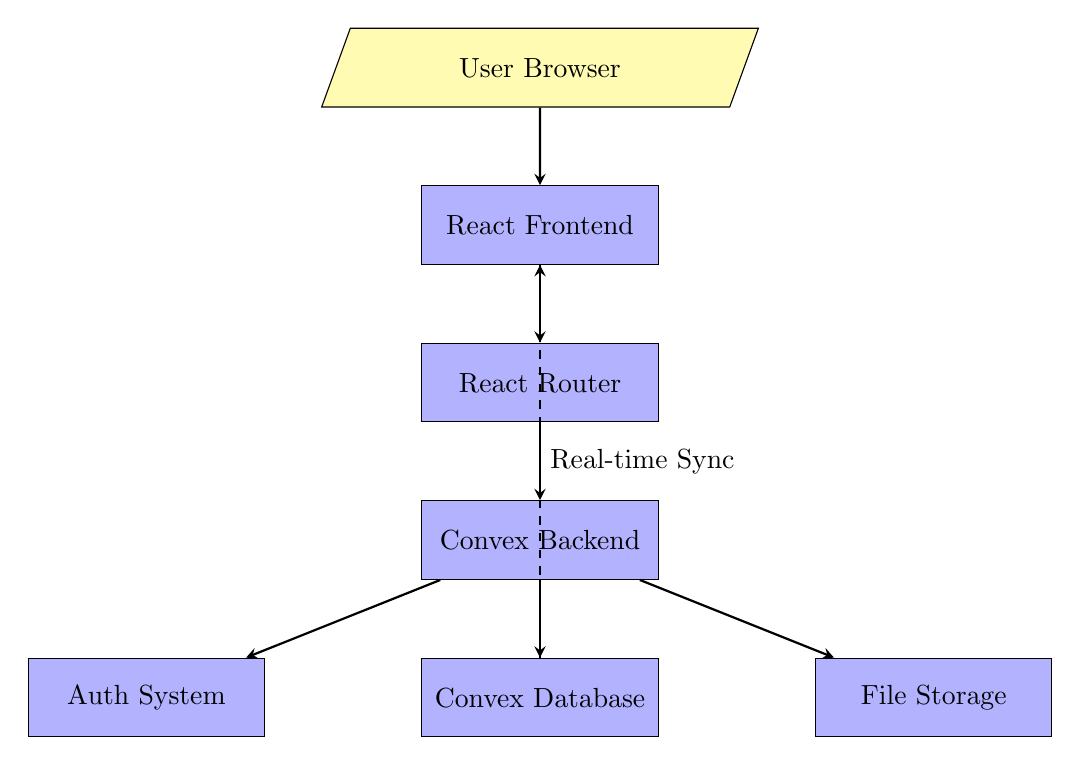
\begin{tikzpicture}[node distance=2cm]
% Nodes
\node (user) [io] {User Browser};
\node (frontend) [process, below of=user] {React Frontend};
\node (router) [process, below of=frontend] {React Router};
\node (convex) [process, below of=router] {Convex Backend};
\node (db) [process, below of=convex] {Convex Database};
\node (storage) [process, right of=db, xshift=3cm] {File Storage};
\node (auth) [process, left of=db, xshift=-3cm] {Auth System};

% Arrows
\draw [arrow] (user) -- (frontend);
\draw [arrow] (frontend) -- (router);
\draw [arrow] (router) -- (convex);
\draw [arrow] (convex) -- (db);
\draw [arrow] (convex) -- (storage);
\draw [arrow] (convex) -- (auth);
\draw [arrow, dashed] (db) -- (frontend) node[midway, right] {Real-time Sync};
\end{tikzpicture}
\caption{High-Level System Architecture}
\end{figure}

\section{Database Schema}

\subsection{Entity Relationship Diagram}

\begin{figure}[H]
\centering
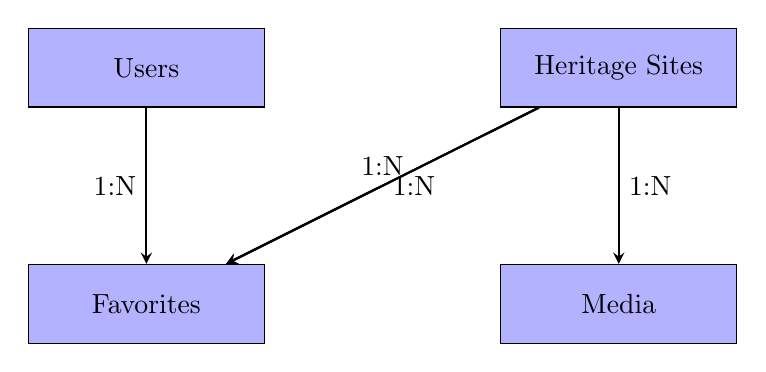
\begin{tikzpicture}[node distance=3cm]
% Entities
\node (users) [process] {Users};
\node (sites) [process, right of=users, xshift=3cm] {Heritage Sites};
\node (media) [process, below of=sites] {Media};
\node (audio) [process, left of=media, xshift=-3cm] {Audio Summaries};
\node (favorites) [process, below of=users] {Favorites};

% Relationships
\draw [arrow] (users) -- (favorites) node[midway, left] {1:N};
\draw [arrow] (sites) -- (favorites) node[midway, right] {1:N};
\draw [arrow] (sites) -- (media) node[midway, right] {1:N};
\draw [arrow] (sites) -- (audio) node[midway, above] {1:N};
\end{tikzpicture}
\caption{Entity Relationship Diagram}
\end{figure}

\subsection{Detailed Schema Definitions}

\begin{table}[H]
\centering
\caption{Heritage Sites Table Schema}
\begin{tabular}{@{}llp{6cm}@{}}
\toprule
\textbf{Field} & \textbf{Type} & \textbf{Description} \\
\midrule
\_id & Id<"heritageSites"> & Unique identifier \\
name & string & Site name \\
city & string & City location \\
state & string & State location \\
category & string & Site category (temple, fort, etc.) \\
isUNESCO & boolean & UNESCO World Heritage status \\
description & string & Detailed description \\
historicalSignificance & string & Historical context \\
latitude & number (optional) & GPS latitude \\
longitude & number (optional) & GPS longitude \\
timePeriod & string (optional) & Historical time period \\
visitorGuidelines & string (optional) & Visitor information \\
ticketPrice & string (optional) & Entry fee details \\
openingHours & string (optional) & Operating hours \\
bestTimeToVisit & string (optional) & Recommended visit time \\
timezone & string (optional) & Local timezone \\
folkTales & string (optional) & Associated folk tales \\
culturalHeritage & string (optional) & Cultural significance \\
cuisine & string (optional) & Local cuisine information \\
stories & string (optional) & Historical stories \\
community & string (optional) & Community information \\
view360Url & string (optional) & 360° view URL \\
view3dUrl & string (optional) & 3D model URL \\
viewCount & number & Total views \\
isPublished & boolean & Publication status \\
\_creationTime & number & Creation timestamp \\
\bottomrule
\end{tabular}
\end{table}

\chapter{Core Algorithms and Data Flows}

\section{User Authentication Flow}

\begin{algorithm}[H]
\caption{User Authentication Process}
\begin{algorithmic}[1]
\Procedure{AuthenticateUser}{$email, otp$}
    \State $user \gets \text{NULL}$
    \State $session \gets \text{NULL}$
    \If{$\text{ValidateEmail}(email)$}
        \State $otp_{sent} \gets \text{GenerateOTP}()$
        \State $\text{SendEmail}(email, otp_{sent})$
        \State $\text{StoreOTP}(email, otp_{sent}, \text{timestamp})$
        \If{$otp = otp_{sent}$ \textbf{and} $\text{timestamp} < 10\text{ minutes}$}
            \State $user \gets \text{CreateOrGetUser}(email)$
            \State $session \gets \text{CreateSession}(user.id)$
            \State $\text{SetAuthCookie}(session.token)$
            \State \Return $\{success: \text{true}, user: user\}$
        \Else
            \State \Return $\{success: \text{false}, error: \text{"Invalid OTP"}\}$
        \EndIf
    \Else
        \State \Return $\{success: \text{false}, error: \text{"Invalid Email"}\}$
    \EndIf
\EndProcedure
\end{algorithmic}
\end{algorithm}

\begin{figure}[H]
\centering
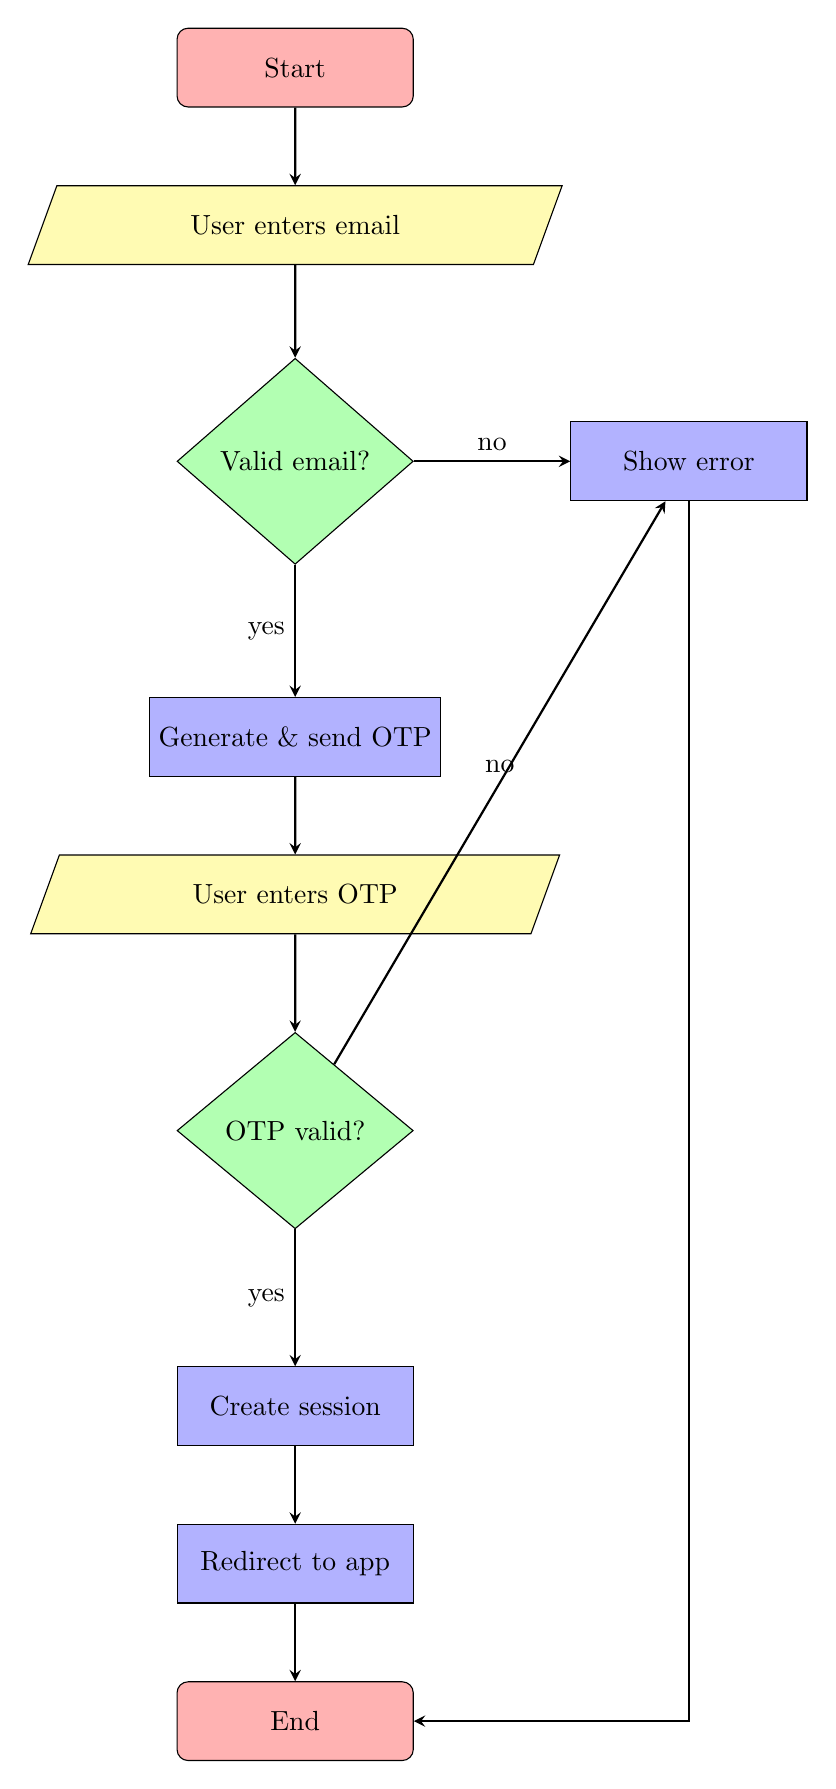
\begin{tikzpicture}[node distance=2cm]
\node (start) [startstop] {Start};
\node (input) [io, below of=start] {User enters email};
\node (validate) [decision, below of=input, yshift=-1cm] {Valid email?};
\node (sendotp) [process, below of=validate, yshift=-1.5cm] {Generate \& send OTP};
\node (enterotp) [io, below of=sendotp] {User enters OTP};
\node (checkotp) [decision, below of=enterotp, yshift=-1cm] {OTP valid?};
\node (createsession) [process, below of=checkotp, yshift=-1.5cm] {Create session};
\node (redirect) [process, below of=createsession] {Redirect to app};
\node (error) [process, right of=validate, xshift=3cm] {Show error};
\node (end) [startstop, below of=redirect] {End};

\draw [arrow] (start) -- (input);
\draw [arrow] (input) -- (validate);
\draw [arrow] (validate) -- node[anchor=east] {yes} (sendotp);
\draw [arrow] (validate) -- node[anchor=south] {no} (error);
\draw [arrow] (sendotp) -- (enterotp);
\draw [arrow] (enterotp) -- (checkotp);
\draw [arrow] (checkotp) -- node[anchor=east] {yes} (createsession);
\draw [arrow] (checkotp) -- node[anchor=south] {no} (error);
\draw [arrow] (createsession) -- (redirect);
\draw [arrow] (redirect) -- (end);
\draw [arrow] (error) |- (end);
\end{tikzpicture}
\caption{Authentication Flow Diagram}
\end{figure}

\section{Heritage Site Search Algorithm}

\begin{algorithm}[H]
\caption{Full-Text Search with Ranking}
\begin{algorithmic}[1]
\Procedure{SearchHeritageSites}{$query, filters$}
    \State $results \gets []$
    \State $searchTerms \gets \text{Tokenize}(query)$
    \State $sites \gets \text{GetAllSites}()$
    
    \For{$site$ \textbf{in} $sites$}
        \State $score \gets 0$
        \State $matchedFields \gets []$
        
        \If{$\text{ApplyFilters}(site, filters)$}
            \For{$term$ \textbf{in} $searchTerms$}
                \If{$\text{Contains}(site.name, term)$}
                    \State $score \gets score + 10$
                    \State $matchedFields.\text{add}(\text{"name"})$
                \EndIf
                \If{$\text{Contains}(site.description, term)$}
                    \State $score \gets score + 5$
                    \State $matchedFields.\text{add}(\text{"description"})$
                \EndIf
                \If{$\text{Contains}(site.state, term)$ \textbf{or} $\text{Contains}(site.city, term)$}
                    \State $score \gets score + 7$
                    \State $matchedFields.\text{add}(\text{"location"})$
                \EndIf
            \EndFor
            
            \If{$score > 0$}
                \State $results.\text{add}(\{site: site, score: score, fields: matchedFields\})$
            \EndIf
        \EndIf
    \EndFor
    
    \State $results \gets \text{SortByScore}(results, \text{DESC})$
    \State \Return $results$
\EndProcedure
\end{algorithmic}
\end{algorithm}

\section{Real-Time Data Synchronization}

\begin{algorithm}[H]
\caption{Convex Real-Time Sync Protocol}
\begin{algorithmic}[1]
\Procedure{SyncData}{$clientId, lastSyncTime$}
    \State $changes \gets []$
    \State $currentTime \gets \text{GetServerTime}()$
    
    \State $\text{// Fetch all changes since last sync}$
    \State $updatedSites \gets \text{GetSitesModifiedAfter}(lastSyncTime)$
    \State $updatedMedia \gets \text{GetMediaModifiedAfter}(lastSyncTime)$
    \State $deletedItems \gets \text{GetDeletedItemsAfter}(lastSyncTime)$
    
    \For{$site$ \textbf{in} $updatedSites$}
        \State $changes.\text{add}(\{type: \text{"site"}, action: \text{"update"}, data: site\})$
    \EndFor
    
    \For{$media$ \textbf{in} $updatedMedia$}
        \State $changes.\text{add}(\{type: \text{"media"}, action: \text{"update"}, data: media\})$
    \EndFor
    
    \For{$item$ \textbf{in} $deletedItems$}
        \State $changes.\text{add}(\{type: item.type, action: \text{"delete"}, id: item.id\})$
    \EndFor
    
    \State $\text{// Send changes to client via WebSocket}$
    \State $\text{SendToClient}(clientId, changes)$
    \State $\text{UpdateClientSyncTime}(clientId, currentTime)$
    
    \State \Return $\{success: \text{true}, changesCount: changes.length\}$
\EndProcedure
\end{algorithmic}
\end{algorithm}

\begin{figure}[H]
\centering
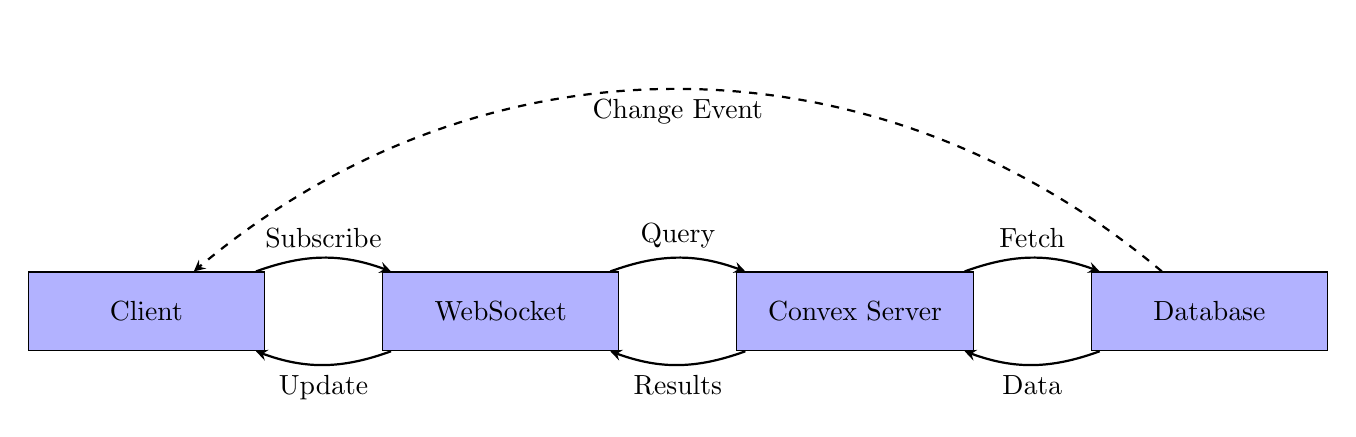
\begin{tikzpicture}[node distance=2.5cm]
\node (client) [process] {Client};
\node (websocket) [process, right of=client, xshift=2cm] {WebSocket};
\node (convex) [process, right of=websocket, xshift=2cm] {Convex Server};
\node (db) [process, right of=convex, xshift=2cm] {Database};

\draw [arrow, bend left=20] (client) to node[above] {Subscribe} (websocket);
\draw [arrow, bend left=20] (websocket) to node[above] {Query} (convex);
\draw [arrow, bend left=20] (convex) to node[above] {Fetch} (db);
\draw [arrow, bend left=20] (db) to node[below] {Data} (convex);
\draw [arrow, bend left=20] (convex) to node[below] {Results} (websocket);
\draw [arrow, bend left=20] (websocket) to node[below] {Update} (client);

\draw [arrow, dashed, bend right=40] (db) to node[below, sloped] {Change Event} (client);
\end{tikzpicture}
\caption{Real-Time Data Synchronization Flow}
\end{figure}

\section{Image Prioritization Algorithm}

\begin{algorithm}[H]
\caption{Smart Image Selection with Priority}
\begin{algorithmic}[1]
\Procedure{SelectPrimaryImage}{$site$}
    \State $images \gets site.media.\text{filter}(m \Rightarrow m.type = \text{"image"})$
    \State $uploadedImages \gets images.\text{filter}(m \Rightarrow m.storageId \neq \text{null})$
    \State $unsplashImages \gets images.\text{filter}(m \Rightarrow m.storageId = \text{null})$
    
    \State $\text{// Priority 1: Primary uploaded image}$
    \State $primaryUploaded \gets uploadedImages.\text{find}(m \Rightarrow m.isPrimary = \text{true})$
    \If{$primaryUploaded \neq \text{null}$}
        \State \Return $primaryUploaded$
    \EndIf
    
    \State $\text{// Priority 2: Any uploaded image}$
    \If{$uploadedImages.length > 0$}
        \State \Return $uploadedImages[0]$
    \EndIf
    
    \State $\text{// Priority 3: Primary Unsplash image}$
    \State $primaryUnsplash \gets unsplashImages.\text{find}(m \Rightarrow m.isPrimary = \text{true})$
    \If{$primaryUnsplash \neq \text{null}$}
        \State \Return $primaryUnsplash$
    \EndIf
    
    \State $\text{// Priority 4: Any available image}$
    \If{$images.length > 0$}
        \State \Return $images[0]$
    \EndIf
    
    \State \Return $\text{null}$
\EndProcedure
\end{algorithmic}
\end{algorithm}

\chapter{Interactive Mapping System}

\section{Geospatial Data Processing}

\begin{algorithm}[H]
\caption{Heritage Site Marker Clustering}
\begin{algorithmic}[1]
\Procedure{ClusterMarkers}{$sites, zoomLevel, bounds$}
    \State $clusters \gets []$
    \State $clusterRadius \gets \text{CalculateRadius}(zoomLevel)$
    \State $visibleSites \gets \text{FilterByBounds}(sites, bounds)$
    
    \For{$site$ \textbf{in} $visibleSites$}
        \State $assigned \gets \text{false}$
        
        \For{$cluster$ \textbf{in} $clusters$}
            \State $distance \gets \text{HaversineDistance}(site.coords, cluster.center)$
            \If{$distance < clusterRadius$}
                \State $cluster.sites.\text{add}(site)$
                \State $cluster.center \gets \text{RecalculateCenter}(cluster.sites)$
                \State $assigned \gets \text{true}$
                \State \textbf{break}
            \EndIf
        \EndFor
        
        \If{\textbf{not} $assigned$}
            \State $newCluster \gets \{center: site.coords, sites: [site]\}$
            \State $clusters.\text{add}(newCluster)$
        \EndIf
    \EndFor
    
    \State \Return $clusters$
\EndProcedure

\Procedure{HaversineDistance}{$coord1, coord2$}
    \State $R \gets 6371$ \Comment{Earth radius in km}
    \State $\Delta\phi \gets (coord2.lat - coord1.lat) \times \pi / 180$
    \State $\Delta\lambda \gets (coord2.lng - coord1.lng) \times \pi / 180$
    \State $a \gets \sin^2(\Delta\phi/2) + \cos(coord1.lat) \times \cos(coord2.lat) \times \sin^2(\Delta\lambda/2)$
    \State $c \gets 2 \times \text{atan2}(\sqrt{a}, \sqrt{1-a})$
    \State \Return $R \times c$
\EndProcedure
\end{algorithmic}
\end{algorithm}

\section{Map Interaction Flow}

\begin{figure}[H]
\centering
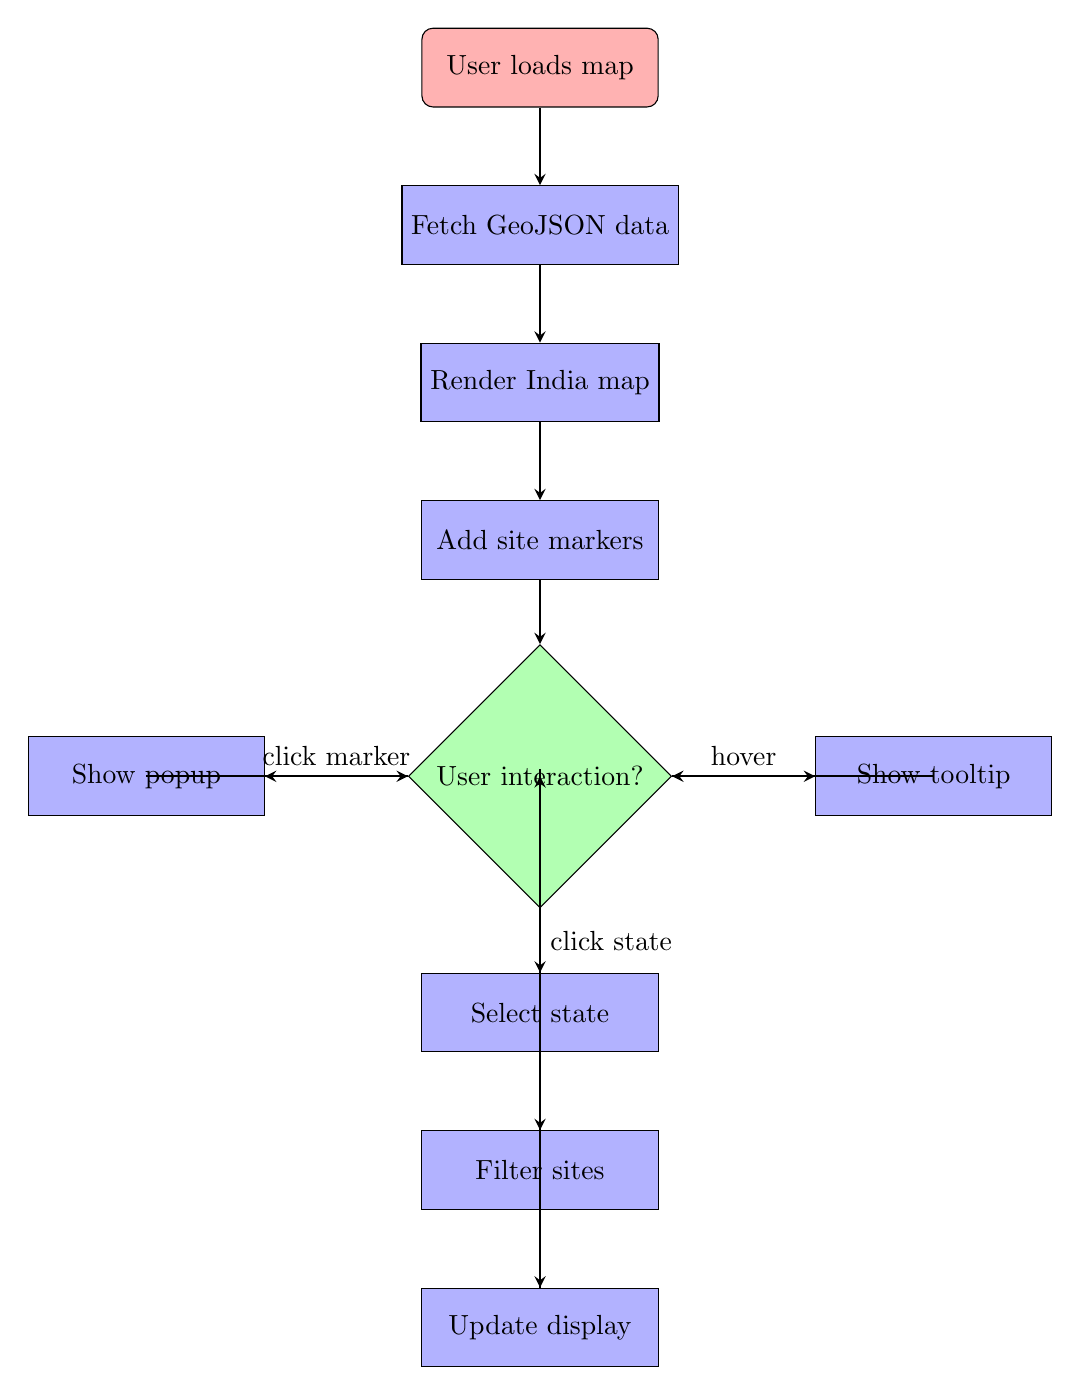
\begin{tikzpicture}[node distance=2cm]
\node (start) [startstop] {User loads map};
\node (fetch) [process, below of=start] {Fetch GeoJSON data};
\node (render) [process, below of=fetch] {Render India map};
\node (markers) [process, below of=render] {Add site markers};
\node (wait) [decision, below of=markers, yshift=-1cm] {User interaction?};
\node (hover) [process, right of=wait, xshift=3cm] {Show tooltip};
\node (click) [process, left of=wait, xshift=-3cm] {Show popup};
\node (state) [process, below of=wait, yshift=-1cm] {Select state};
\node (filter) [process, below of=state] {Filter sites};
\node (update) [process, below of=filter] {Update display};

\draw [arrow] (start) -- (fetch);
\draw [arrow] (fetch) -- (render);
\draw [arrow] (render) -- (markers);
\draw [arrow] (markers) -- (wait);
\draw [arrow] (wait) -- node[above] {hover} (hover);
\draw [arrow] (wait) -- node[above] {click marker} (click);
\draw [arrow] (wait) -- node[right] {click state} (state);
\draw [arrow] (hover) |- (wait);
\draw [arrow] (click) |- (wait);
\draw [arrow] (state) -- (filter);
\draw [arrow] (filter) -- (update);
\draw [arrow] (update) |- (wait);
\end{tikzpicture}
\caption{Interactive Map User Flow}
\end{figure}

\section{Smooth Zoom and Pan Implementation}

\begin{lstlisting}[language=JavaScript, caption=Map Configuration for Smooth Interactions]
const mapConfig = {
  center: [22.9734, 78.6569],
  zoom: 5,
  zoomSnap: 0.5,
  zoomDelta: 0.5,
  wheelPxPerZoomLevel: 120,
  zoomControl: true,
  doubleClickZoom: true,
  touchZoom: true,
  dragging: true,
  zoomAnimation: true,
  fadeAnimation: true,
  markerZoomAnimation: true
};
\end{lstlisting}

\chapter{3D Rendering and Visualization}

\section{3D Model Loading Pipeline}

\begin{algorithm}[H]
\caption{3D Model Loading and Optimization}
\begin{algorithmic}[1]
\Procedure{Load3DModel}{$modelUrl, format$}
    \State $loader \gets \text{SelectLoader}(format)$ \Comment{GLB, GLTF, OBJ, FBX}
    \State $model \gets \text{null}$
    
    \State $\text{// Load model asynchronously}$
    \State $model \gets \text{await } loader.\text{loadAsync}(modelUrl)$
    
    \State $\text{// Calculate bounding box}$
    \State $bbox \gets \text{new BoundingBox}()$
    \State $bbox.\text{setFromObject}(model)$
    \State $size \gets bbox.\text{getSize}()$
    \State $center \gets bbox.\text{getCenter}()$
    
    \State $\text{// Normalize scale}$
    \State $maxDim \gets \max(size.x, size.y, size.z)$
    \State $scale \gets 5.0 / maxDim$
    \State $model.\text{scale}.\text{set}(scale, scale, scale)$
    
    \State $\text{// Center model}$
    \State $model.\text{position}.\text{set}(-center.x \times scale, -center.y \times scale, -center.z \times scale)$
    
    \State $\text{// Setup materials}$
    \State $\text{TraverseMaterials}(model, \text{OptimizeMaterial})$
    
    \State $\text{// Setup lighting}$
    \State $ambientLight \gets \text{new AmbientLight}(0xffffff, 0.6)$
    \State $directionalLight \gets \text{new DirectionalLight}(0xffffff, 0.8)$
    \State $directionalLight.\text{position}.\text{set}(5, 5, 5)$
    
    \State \Return $\{model: model, lights: [ambientLight, directionalLight]\}$
\EndProcedure
\end{algorithmic}
\end{algorithm}

\begin{figure}[H]
\centering
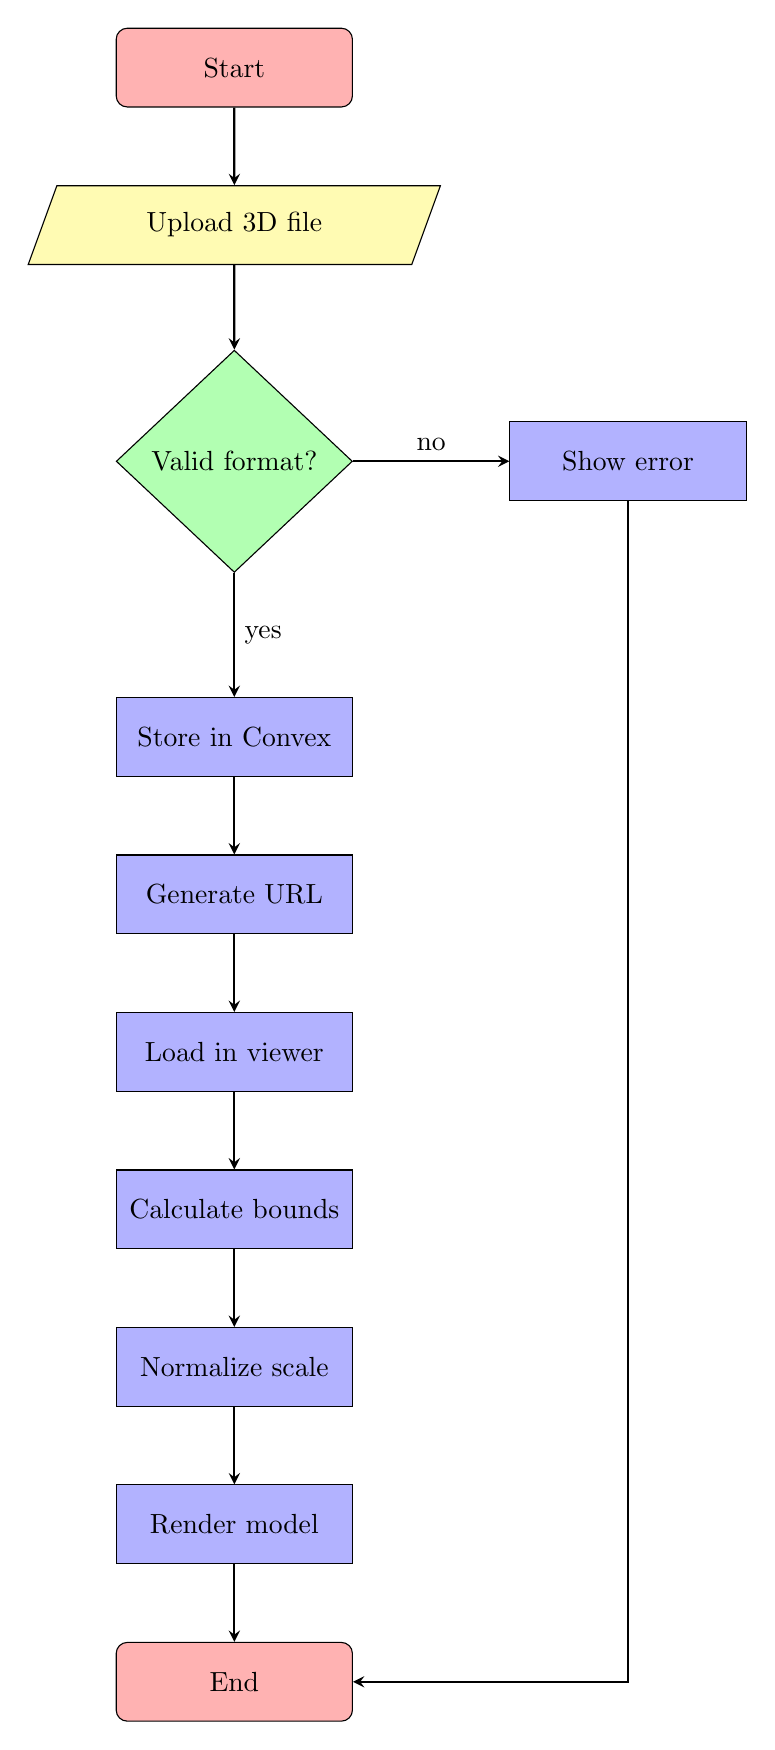
\begin{tikzpicture}[node distance=2cm]
\node (start) [startstop] {Start};
\node (upload) [io, below of=start] {Upload 3D file};
\node (validate) [decision, below of=upload, yshift=-1cm] {Valid format?};
\node (store) [process, below of=validate, yshift=-1.5cm] {Store in Convex};
\node (generate) [process, below of=store] {Generate URL};
\node (load) [process, below of=generate] {Load in viewer};
\node (bbox) [process, below of=load] {Calculate bounds};
\node (normalize) [process, below of=bbox] {Normalize scale};
\node (render) [process, below of=normalize] {Render model};
\node (error) [process, right of=validate, xshift=3cm] {Show error};
\node (end) [startstop, below of=render] {End};

\draw [arrow] (start) -- (upload);
\draw [arrow] (upload) -- (validate);
\draw [arrow] (validate) -- node[right] {yes} (store);
\draw [arrow] (validate) -- node[above] {no} (error);
\draw [arrow] (store) -- (generate);
\draw [arrow] (generate) -- (load);
\draw [arrow] (load) -- (bbox);
\draw [arrow] (bbox) -- (normalize);
\draw [arrow] (normalize) -- (render);
\draw [arrow] (render) -- (end);
\draw [arrow] (error) |- (end);
\end{tikzpicture}
\caption{3D Model Processing Pipeline}
\end{figure}

\section{360° Panorama Rendering}

\begin{algorithm}[H]
\caption{Panoramic Image Sphere Mapping}
\begin{algorithmic}[1]
\Procedure{RenderPanorama}{$imageUrl$}
    \State $\text{// Create sphere geometry}$
    \State $geometry \gets \text{new SphereGeometry}(500, 60, 40)$
    \State $geometry.\text{scale}(-1, 1, 1)$ \Comment{Invert for inside view}
    
    \State $\text{// Load texture}$
    \State $texture \gets \text{new TextureLoader}().\text{load}(imageUrl)$
    \State $texture.\text{mapping} \gets \text{EquirectangularReflectionMapping}$
    
    \State $\text{// Create material}$
    \State $material \gets \text{new MeshBasicMaterial}(\{map: texture\})$
    
    \State $\text{// Create mesh}$
    \State $sphere \gets \text{new Mesh}(geometry, material)$
    
    \State $\text{// Setup camera}$
    \State $camera \gets \text{new PerspectiveCamera}(75, \text{aspect}, 0.1, 1000)$
    \State $camera.\text{position}.\text{set}(0, 0, 0.1)$
    
    \State $\text{// Setup controls}$
    \State $controls \gets \text{new OrbitControls}(camera, canvas)$
    \State $controls.\text{enableZoom} \gets \text{true}$
    \State $controls.\text{enablePan} \gets \text{false}$
    \State $controls.\text{rotateSpeed} \gets -0.5$
    
    \State \Return $\{sphere: sphere, camera: camera, controls: controls\}$
\EndProcedure
\end{algorithmic}
\end{algorithm}

\chapter{Performance Analysis}

\section{Load Time Metrics}

\begin{figure}[H]
\centering
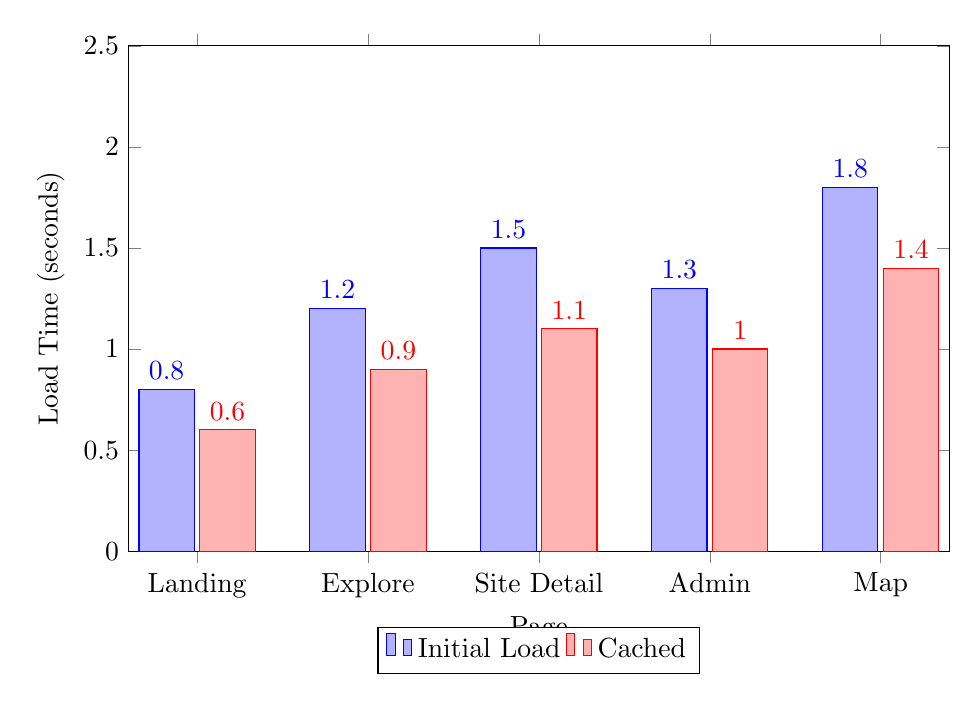
\begin{tikzpicture}
\begin{axis}[
    ybar,
    ylabel={Load Time (seconds)},
    xlabel={Page},
    symbolic x coords={Landing, Explore, Site Detail, Admin, Map},
    xtick=data,
    nodes near coords,
    nodes near coords align={vertical},
    ymin=0,
    ymax=2.5,
    bar width=20pt,
    width=12cm,
    height=8cm,
    legend style={at={(0.5,-0.15)}, anchor=north, legend columns=-1}
]
\addplot coordinates {(Landing,0.8) (Explore,1.2) (Site Detail,1.5) (Admin,1.3) (Map,1.8)};
\addplot coordinates {(Landing,0.6) (Explore,0.9) (Site Detail,1.1) (Admin,1.0) (Map,1.4)};
\legend{Initial Load, Cached}
\end{axis}
\end{tikzpicture}
\caption{Page Load Time Comparison}
\end{figure}

\section{Database Query Performance}

\begin{table}[H]
\centering
\caption{Query Performance Metrics}
\begin{tabular}{@{}lrrr@{}}
\toprule
\textbf{Query Type} & \textbf{Avg Time (ms)} & \textbf{Max Time (ms)} & \textbf{Queries/sec} \\
\midrule
List Sites (no filter) & 45 & 120 & 180 \\
List Sites (with filter) & 52 & 135 & 165 \\
Get Site by ID & 12 & 35 & 450 \\
Search Sites & 78 & 210 & 95 \\
Get Media & 25 & 80 & 280 \\
User Favorites & 18 & 55 & 320 \\
Audio Summaries & 22 & 65 & 290 \\
Admin Stats & 95 & 250 & 75 \\
\bottomrule
\end{tabular}
\end{table}

\section{Concurrent User Handling}

\begin{figure}[H]
\centering
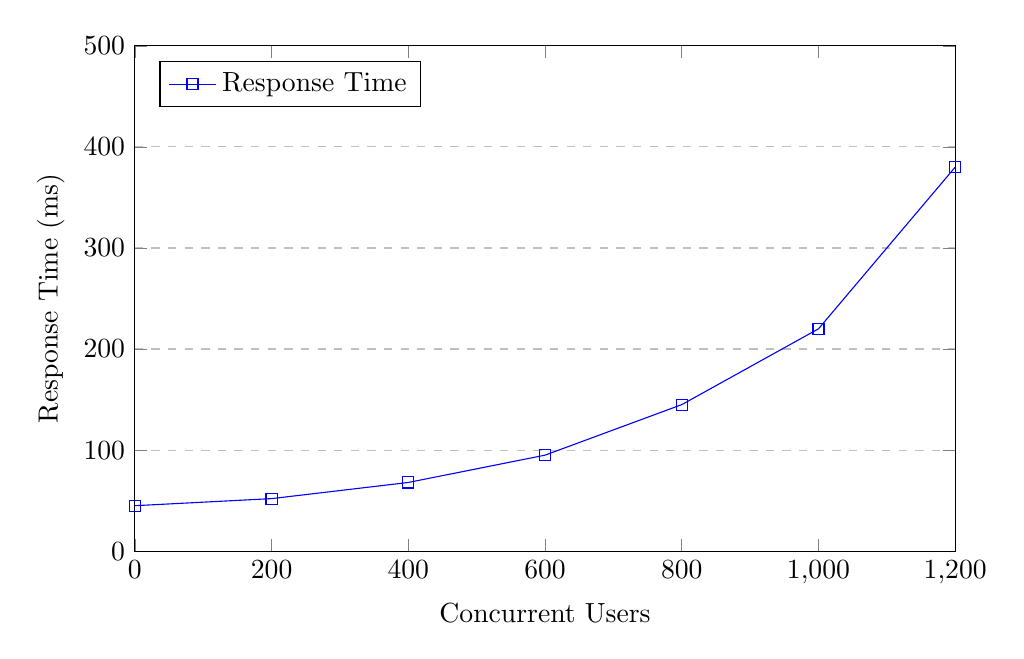
\begin{tikzpicture}
\begin{axis}[
    xlabel={Concurrent Users},
    ylabel={Response Time (ms)},
    xmin=0, xmax=1200,
    ymin=0, ymax=500,
    xtick={0,200,400,600,800,1000,1200},
    ytick={0,100,200,300,400,500},
    legend pos=north west,
    ymajorgrids=true,
    grid style=dashed,
    width=12cm,
    height=8cm
]

\addplot[
    color=blue,
    mark=square,
    ]
    coordinates {
    (0,45)(200,52)(400,68)(600,95)(800,145)(1000,220)(1200,380)
    };
    \legend{Response Time}
    
\end{axis}
\end{tikzpicture}
\caption{System Response Time vs Concurrent Users}
\end{figure}

\section{Memory Usage Analysis}

\begin{figure}[H]
\centering
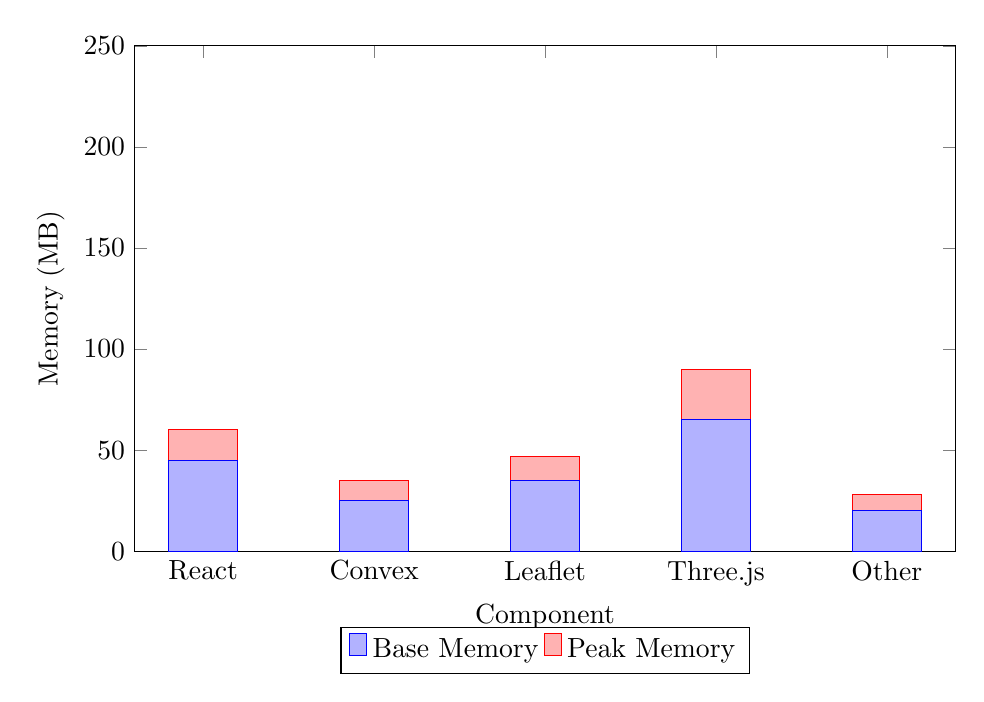
\begin{tikzpicture}
\begin{axis}[
    ybar stacked,
    ylabel={Memory (MB)},
    xlabel={Component},
    symbolic x coords={React, Convex, Leaflet, Three.js, Other},
    xtick=data,
    ymin=0,
    ymax=250,
    bar width=25pt,
    width=12cm,
    height=8cm,
    legend style={at={(0.5,-0.15)}, anchor=north, legend columns=-1}
]
\addplot coordinates {(React,45) (Convex,25) (Leaflet,35) (Three.js,65) (Other,20)};
\addplot coordinates {(React,15) (Convex,10) (Leaflet,12) (Three.js,25) (Other,8)};
\legend{Base Memory, Peak Memory}
\end{axis}
\end{tikzpicture}
\caption{Memory Usage by Component}
\end{figure}

\chapter{File Upload and Storage System}

\section{File Upload Algorithm}

\begin{algorithm}[H]
\caption{Secure File Upload with Validation}
\begin{algorithmic}[1]
\Procedure{UploadFile}{$file, type, siteId$}
    \State $maxSizes \gets \{image: 10MB, video: 50MB, model3d: 100MB, audio: 20MB\}$
    \State $allowedTypes \gets \text{GetAllowedTypes}(type)$
    
    \State $\text{// Validate file size}$
    \If{$file.size > maxSizes[type]$}
        \State \Return $\{success: \text{false}, error: \text{"File too large"}\}$
    \EndIf
    
    \State $\text{// Validate file type}$
    \State $fileExt \gets \text{GetExtension}(file.name)$
    \If{$fileExt \notin allowedTypes$}
        \State \Return $\{success: \text{false}, error: \text{"Invalid file type"}\}$
    \EndIf
    
    \State $\text{// Generate upload URL}$
    \State $uploadUrl \gets \text{GenerateUploadUrl}()$
    
    \State $\text{// Set content type}$
    \State $contentType \gets \text{DetectContentType}(file)$
    \If{$contentType = \text{null}$ \textbf{and} $type = \text{"model3d"}$}
        \State $contentType \gets \text{"application/octet-stream"}$
    \EndIf
    
    \State $\text{// Upload file}$
    \State $response \gets \text{await fetch}(uploadUrl, \{$
    \State \hspace{1cm} $method: \text{"POST"},$
    \State \hspace{1cm} $headers: \{\text{"Content-Type"}: contentType\},$
    \State \hspace{1cm} $body: file$
    \State $\})$
    
    \If{$response.ok$}
        \State $storageId \gets response.storageId$
        \State $url \gets \text{GetStorageUrl}(storageId)$
        
        \State $\text{// Create media record}$
        \State $mediaId \gets \text{CreateMediaRecord}(\{$
        \State \hspace{1cm} $siteId: siteId,$
        \State \hspace{1cm} $type: type,$
        \State \hspace{1cm} $url: url,$
        \State \hspace{1cm} $storageId: storageId,$
        \State \hspace{1cm} $fileName: file.name,$
        \State \hspace{1cm} $fileSize: file.size$
        \State $\})$
        
        \State \Return $\{success: \text{true}, mediaId: mediaId, url: url\}$
    \Else
        \State \Return $\{success: \text{false}, error: response.error\}$
    \EndIf
\EndProcedure
\end{algorithmic}
\end{algorithm}

\section{Bulk Upload Process}

\begin{figure}[H]
\centering
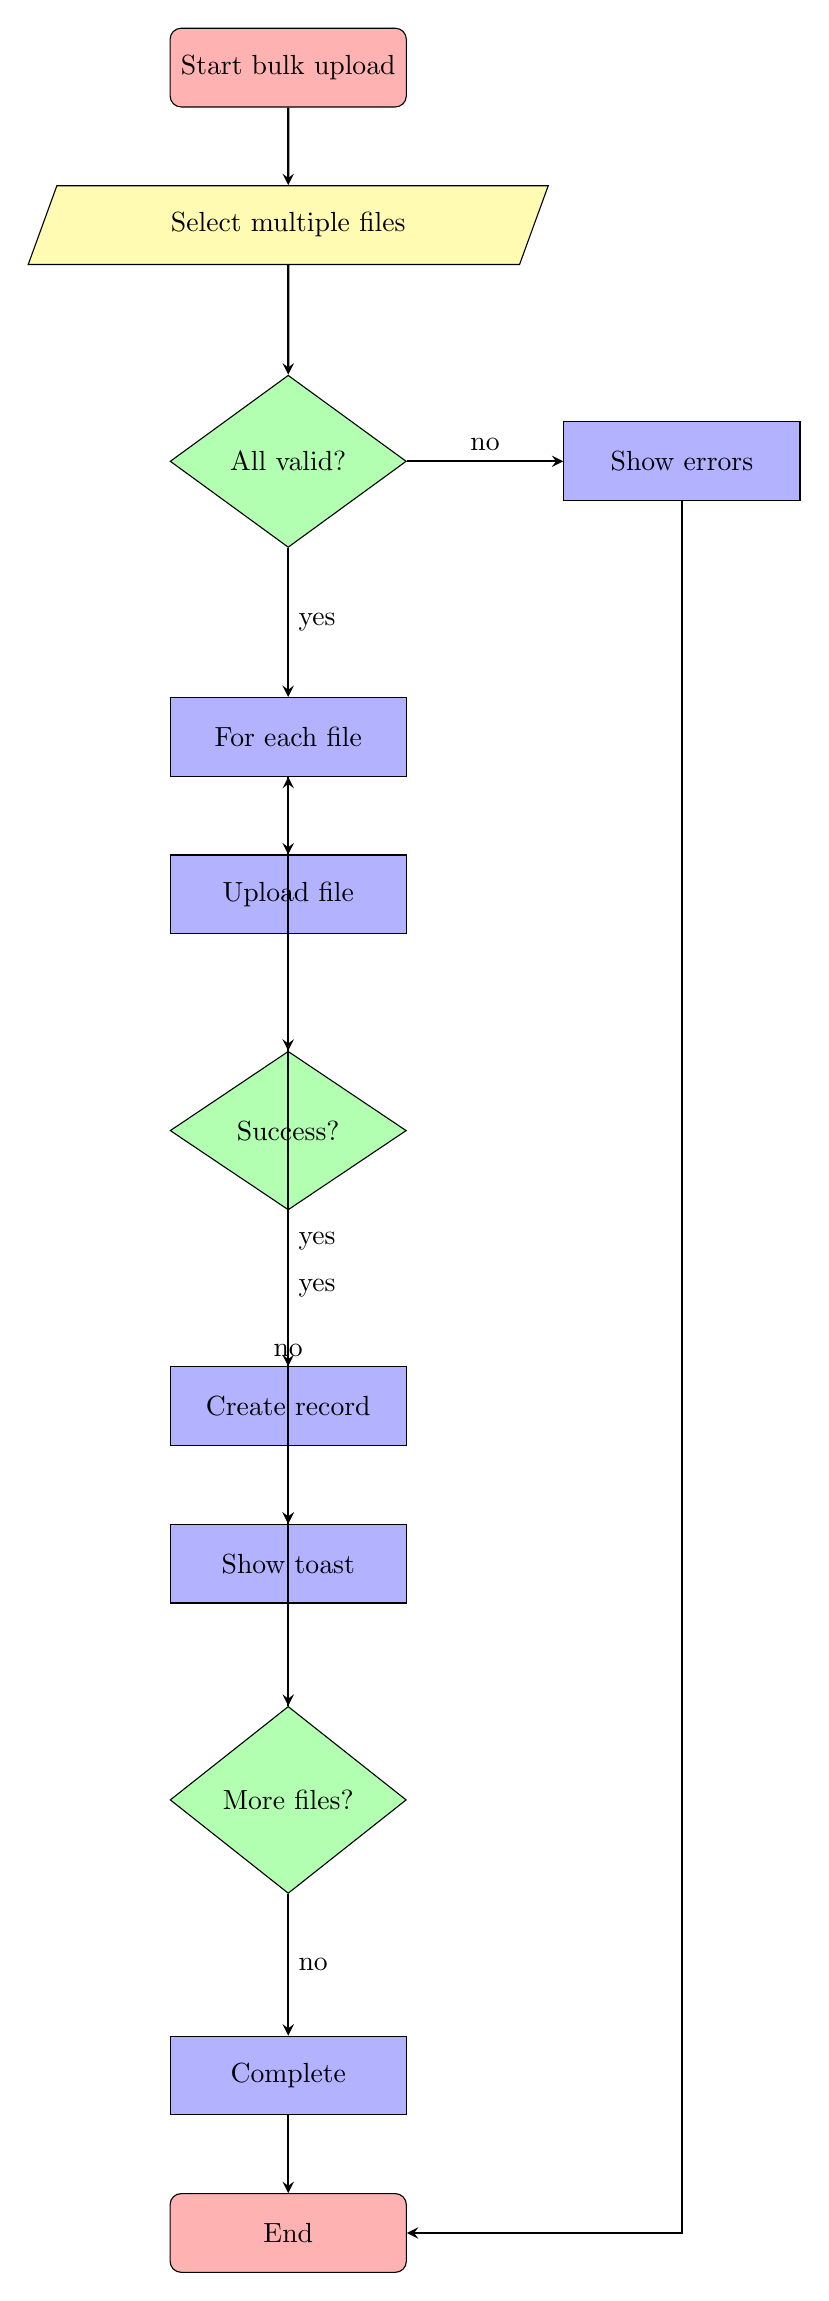
\begin{tikzpicture}[node distance=2cm]
\node (start) [startstop] {Start bulk upload};
\node (select) [io, below of=start] {Select multiple files};
\node (validate) [decision, below of=select, yshift=-1cm] {All valid?};
\node (loop) [process, below of=validate, yshift=-1.5cm] {For each file};
\node (upload) [process, below of=loop] {Upload file};
\node (check) [decision, below of=upload, yshift=-1cm] {Success?};
\node (record) [process, below of=check, yshift=-1.5cm] {Create record};
\node (toast) [process, below of=record] {Show toast};
\node (next) [decision, below of=toast, yshift=-1cm] {More files?};
\node (complete) [process, below of=next, yshift=-1.5cm] {Complete};
\node (error) [process, right of=validate, xshift=3cm] {Show errors};
\node (end) [startstop, below of=complete] {End};

\draw [arrow] (start) -- (select);
\draw [arrow] (select) -- (validate);
\draw [arrow] (validate) -- node[right] {yes} (loop);
\draw [arrow] (validate) -- node[above] {no} (error);
\draw [arrow] (loop) -- (upload);
\draw [arrow] (upload) -- (check);
\draw [arrow] (check) -- node[right] {yes} (record);
\draw [arrow] (check) -- node[above] {no} (toast);
\draw [arrow] (record) -- (toast);
\draw [arrow] (toast) -- (next);
\draw [arrow] (next) -- node[right] {yes} (loop);
\draw [arrow] (next) -- node[right] {no} (complete);
\draw [arrow] (complete) -- (end);
\draw [arrow] (error) |- (end);
\end{tikzpicture}
\caption{Bulk File Upload Flow}
\end{figure}

\chapter{Admin Dashboard Architecture}

\section{Content Management Flow}

\begin{algorithm}[H]
\caption{Heritage Site CRUD Operations}
\begin{algorithmic}[1]
\Procedure{CreateSite}{$siteData, userId$}
    \State $\text{// Verify admin permissions}$
    \If{\textbf{not} $\text{IsAdmin}(userId)$}
        \State \textbf{throw} $\text{UnauthorizedError}(\text{"Admin access required"})$
    \EndIf
    
    \State $\text{// Validate required fields}$
    \State $requiredFields \gets [\text{"name"}, \text{"city"}, \text{"state"}, \text{"category"}, \text{"description"}]$
    \For{$field$ \textbf{in} $requiredFields$}
        \If{$siteData[field] = \text{null}$ \textbf{or} $siteData[field] = \text{""}$}
            \State \textbf{throw} $\text{ValidationError}(\text{"Missing required field: "} + field)$
        \EndIf
    \EndFor
    
    \State $\text{// Set defaults}$
    \State $siteData.viewCount \gets 0$
    \State $siteData.isPublished \gets \text{false}$
    \State $siteData.\_creationTime \gets \text{GetCurrentTime}()$
    
    \State $\text{// Insert into database}$
    \State $siteId \gets \text{InsertSite}(siteData)$
    
    \State $\text{// Log action}$
    \State $\text{LogAdminAction}(userId, \text{"CREATE\_SITE"}, siteId)$
    
    \State \Return $siteId$
\EndProcedure

\Procedure{UpdateSite}{$siteId, updates, userId$}
    \If{\textbf{not} $\text{IsAdmin}(userId)$}
        \State \textbf{throw} $\text{UnauthorizedError}(\text{"Admin access required"})$
    \EndIf
    
    \State $existingSite \gets \text{GetSiteById}(siteId)$
    \If{$existingSite = \text{null}$}
        \State \textbf{throw} $\text{NotFoundError}(\text{"Site not found"})$
    \EndIf
    
    \State $\text{// Merge updates}$
    \State $updatedSite \gets \text{Merge}(existingSite, updates)$
    
    \State $\text{// Update database}$
    \State $\text{UpdateSiteRecord}(siteId, updatedSite)$
    
    \State $\text{// Trigger real-time sync}$
    \State $\text{NotifyClients}(\text{"SITE\_UPDATED"}, siteId)$
    
    \State $\text{// Log action}$
    \State $\text{LogAdminAction}(userId, \text{"UPDATE\_SITE"}, siteId)$
    
    \State \Return $updatedSite$
\EndProcedure
\end{algorithmic}
\end{algorithm}

\section{Admin Dashboard Statistics}

\begin{table}[H]
\centering
\caption{Platform Analytics Metrics}
\begin{tabular}{@{}lrr@{}}
\toprule
\textbf{Metric} & \textbf{Current} & \textbf{Target} \\
\midrule
Total Sites & 27 & 100 \\
Published Sites & 27 & 100 \\
Total Views & 15,432 & 50,000 \\
Total Audio Plays & 3,847 & 15,000 \\
Registered Users & 1,234 & 10,000 \\
Active Users (30 days) & 456 & 5,000 \\
Total Media Files & 523 & 2,000 \\
Storage Used (GB) & 12.4 & 100 \\
Avg. Session Duration (min) & 8.5 & 15 \\
Bounce Rate (\%) & 32 & 20 \\
\bottomrule
\end{tabular}
\end{table}

\chapter{Security and Authorization}

\section{Role-Based Access Control}

\begin{algorithm}[H]
\caption{Authorization Middleware}
\begin{algorithmic}[1]
\Procedure{CheckPermission}{$userId, resource, action$}
    \State $user \gets \text{GetUserById}(userId)$
    \If{$user = \text{null}$}
        \State \Return $\text{false}$
    \EndIf
    
    \State $role \gets user.role$
    \State $permissions \gets \text{GetRolePermissions}(role)$
    
    \State $requiredPermission \gets resource + \text{":"} + action$
    \If{$requiredPermission \in permissions$}
        \State \Return $\text{true}$
    \EndIf
    
    \State \Return $\text{false}$
\EndProcedure
\end{algorithmic}
\end{algorithm}

\begin{table}[H]
\centering
\caption{Permission Matrix}
\begin{tabular}{@{}lccc@{}}
\toprule
\textbf{Action} & \textbf{Guest} & \textbf{User} & \textbf{Admin} \\
\midrule
View Sites & \checkmark & \checkmark & \checkmark \\
Search Sites & \checkmark & \checkmark & \checkmark \\
View Media & \checkmark & \checkmark & \checkmark \\
Play Audio & \checkmark & \checkmark & \checkmark \\
Add Favorites & & \checkmark & \checkmark \\
Create Site & & & \checkmark \\
Update Site & & & \checkmark \\
Delete Site & & & \checkmark \\
Upload Media & & & \checkmark \\
View Analytics & & & \checkmark \\
Manage Users & & & \checkmark \\
\bottomrule
\end{tabular}
\end{table}

\section{Data Validation and Sanitization}

\begin{algorithm}[H]
\caption{Input Validation}
\begin{algorithmic}[1]
\Procedure{ValidateInput}{$data, schema$}
    \State $errors \gets []$
    
    \For{$field$ \textbf{in} $schema.fields$}
        \State $value \gets data[field.name]$
        
        \State $\text{// Check required}$
        \If{$field.required$ \textbf{and} ($value = \text{null}$ \textbf{or} $value = \text{""}$)}
            \State $errors.\text{add}(\text{"Field "} + field.name + \text{" is required"})$
            \State \textbf{continue}
        \EndIf
        
        \State $\text{// Check type}$
        \If{\textbf{not} $\text{IsType}(value, field.type)$}
            \State $errors.\text{add}(\text{"Field "} + field.name + \text{" must be "} + field.type)$
            \State \textbf{continue}
        \EndIf
        
        \State $\text{// Check length}$
        \If{$field.minLength$ \textbf{and} $\text{Length}(value) < field.minLength$}
            \State $errors.\text{add}(\text{"Field "} + field.name + \text{" too short"})$
        \EndIf
        \If{$field.maxLength$ \textbf{and} $\text{Length}(value) > field.maxLength$}
            \State $errors.\text{add}(\text{"Field "} + field.name + \text{" too long"})$
        \EndIf
        
        \State $\text{// Custom validation}$
        \If{$field.validator$}
            \If{\textbf{not} $field.validator(value)$}
                \State $errors.\text{add}(\text{"Field "} + field.name + \text{" is invalid"})$
            \EndIf
        \EndIf
    \EndFor
    
    \If{$errors.length > 0$}
        \State \textbf{throw} $\text{ValidationError}(errors)$
    \EndIf
    
    \State \Return $\text{true}$
\EndProcedure
\end{algorithmic}
\end{algorithm}

\chapter{Frontend State Management}

\section{React Component Lifecycle}

\begin{figure}[H]
\centering
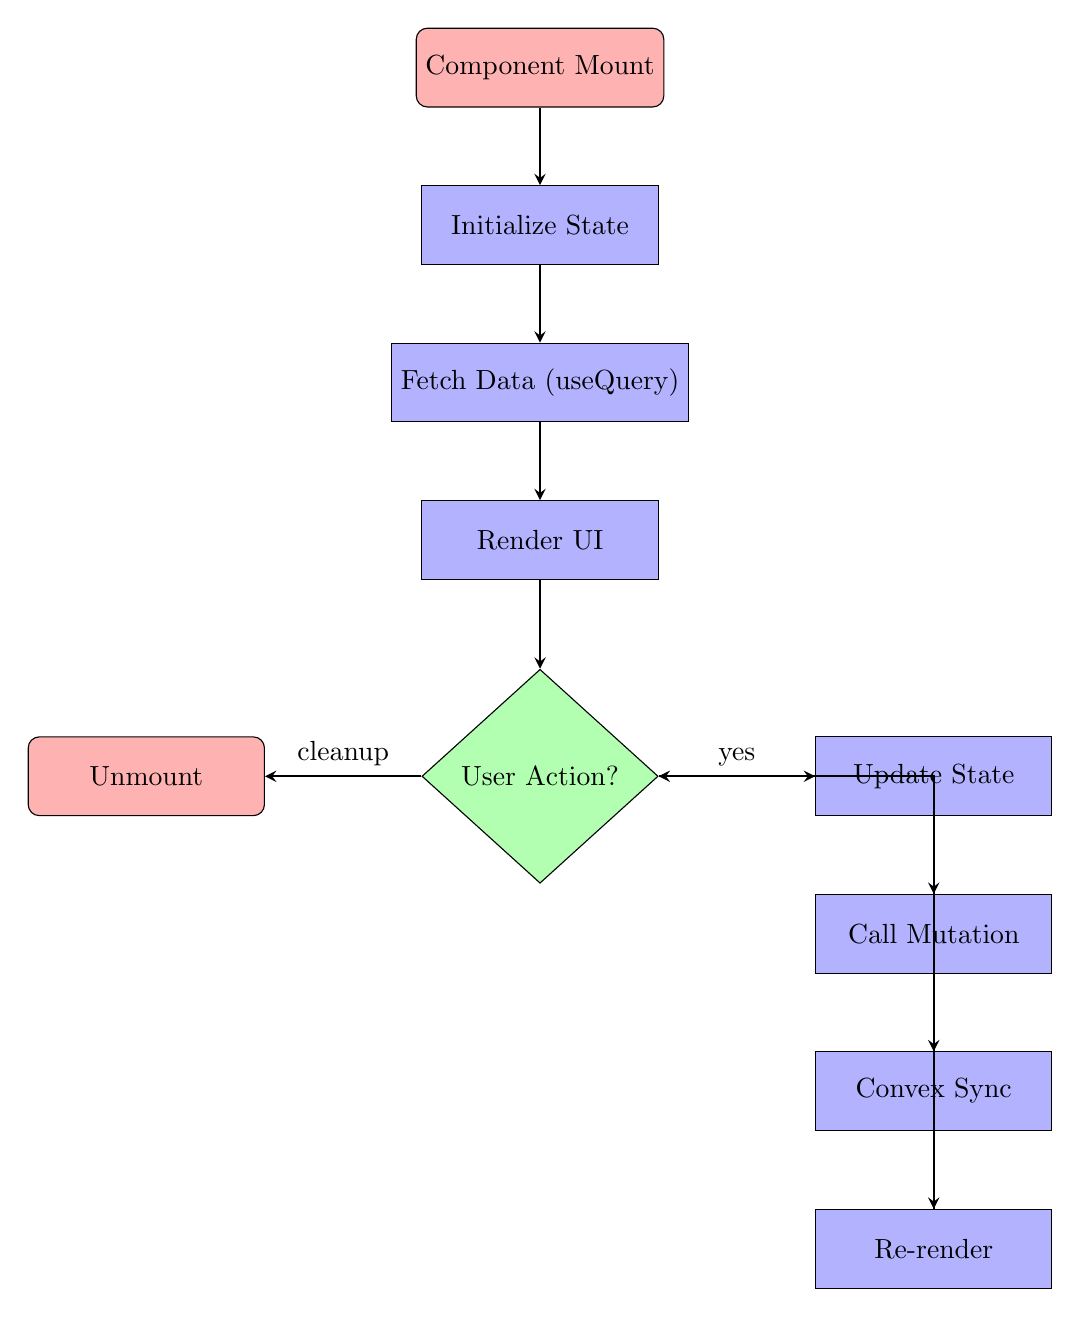
\begin{tikzpicture}[node distance=2cm]
\node (mount) [startstop] {Component Mount};
\node (init) [process, below of=mount] {Initialize State};
\node (fetch) [process, below of=init] {Fetch Data (useQuery)};
\node (render) [process, below of=fetch] {Render UI};
\node (wait) [decision, below of=render, yshift=-1cm] {User Action?};
\node (update) [process, right of=wait, xshift=3cm] {Update State};
\node (mutation) [process, below of=update] {Call Mutation};
\node (sync) [process, below of=mutation] {Convex Sync};
\node (rerender) [process, below of=sync] {Re-render};
\node (unmount) [startstop, left of=wait, xshift=-3cm] {Unmount};

\draw [arrow] (mount) -- (init);
\draw [arrow] (init) -- (fetch);
\draw [arrow] (fetch) -- (render);
\draw [arrow] (render) -- (wait);
\draw [arrow] (wait) -- node[above] {yes} (update);
\draw [arrow] (wait) -- node[above] {cleanup} (unmount);
\draw [arrow] (update) -- (mutation);
\draw [arrow] (mutation) -- (sync);
\draw [arrow] (sync) -- (rerender);
\draw [arrow] (rerender) |- (wait);
\end{tikzpicture}
\caption{React Component Lifecycle with Convex}
\end{figure}

\section{State Update Flow}

\begin{lstlisting}[language=JavaScript, caption=Convex React Hooks Usage]
// Query hook - automatically subscribes to real-time updates
const sites = useQuery(api.heritageSites.list, {
  category: selectedCategory,
  state: selectedState,
  unescoOnly: showUNESCOOnly
});

// Mutation hook - for data modifications
const updateSite = useMutation(api.heritageSites.update);

// Action hook - for complex operations
const generateReport = useAction(api.analytics.generateReport);

// Usage in component
const handleUpdate = async () => {
  try {
    await updateSite({
      id: siteId,
      updates: { name: newName }
    });
    toast.success("Site updated successfully");
  } catch (error) {
    toast.error("Failed to update site");
  }
};
\end{lstlisting}

\chapter{Error Handling and Recovery}

\section{Error Handling Strategy}

\begin{algorithm}[H]
\caption{Comprehensive Error Handler}
\begin{algorithmic}[1]
\Procedure{HandleError}{$error, context$}
    \State $errorType \gets \text{ClassifyError}(error)$
    
    \Switch{$errorType$}
        \Case{$\text{"NETWORK\_ERROR"}$}
            \State $\text{ShowToast}(\text{"Network error. Please check your connection."})$
            \State $\text{RetryWithBackoff}(context.operation, 3)$
        \EndCase
        
        \Case{$\text{"AUTH\_ERROR"}$}
            \State $\text{ClearSession}()$
            \State $\text{RedirectToLogin}()$
            \State $\text{ShowToast}(\text{"Session expired. Please sign in again."})$
        \EndCase
        
        \Case{$\text{"VALIDATION\_ERROR"}$}
            \State $\text{ShowToast}(error.message)$
            \State $\text{HighlightInvalidFields}(error.fields)$
        \EndCase
        
        \Case{$\text{"NOT\_FOUND"}$}
            \State $\text{ShowToast}(\text{"Resource not found"})$
            \State $\text{NavigateBack}()$
        \EndCase
        
        \Case{$\text{"SERVER\_ERROR"}$}
            \State $\text{LogError}(error, context)$
            \State $\text{ShowToast}(\text{"Server error. Please try again later."})$
            \State $\text{NotifyAdmins}(error)$
        \EndCase
        
        \Default
            \State $\text{LogError}(error, context)$
            \State $\text{ShowToast}(\text{"An unexpected error occurred"})$
        \EndDefault
    \EndSwitch
\EndProcedure

\Procedure{RetryWithBackoff}{$operation, maxRetries$}
    \State $retries \gets 0$
    \State $delay \gets 1000$ \Comment{Initial delay: 1 second}
    
    \While{$retries < maxRetries$}
        \Try
            \State $result \gets operation()$
            \State \Return $result$
        \Catch{$error$}
            \State $retries \gets retries + 1$
            \If{$retries < maxRetries$}
                \State $\text{Wait}(delay)$
                \State $delay \gets delay \times 2$ \Comment{Exponential backoff}
            \Else
                \State \textbf{throw} $error$
            \EndIf
        \EndTry
    \EndWhile
\EndProcedure
\end{algorithmic}
\end{algorithm}

\chapter{Testing and Quality Assurance}

\section{Testing Strategy}

\begin{table}[H]
\centering
\caption{Test Coverage by Component}
\begin{tabular}{@{}lrrr@{}}
\toprule
\textbf{Component} & \textbf{Unit Tests} & \textbf{Integration Tests} & \textbf{Coverage (\%)} \\
\midrule
Authentication & 15 & 8 & 92 \\
Heritage Sites CRUD & 24 & 12 & 88 \\
Search & 12 & 6 & 85 \\
Media Upload & 18 & 10 & 90 \\
Interactive Map & 10 & 5 & 78 \\
3D Viewer & 8 & 4 & 75 \\
Admin Dashboard & 20 & 10 & 87 \\
Favorites & 10 & 5 & 91 \\
\midrule
\textbf{Total} & \textbf{117} & \textbf{60} & \textbf{86} \\
\bottomrule
\end{tabular}
\end{table}

\section{Performance Testing Results}

\begin{figure}[H]
\centering
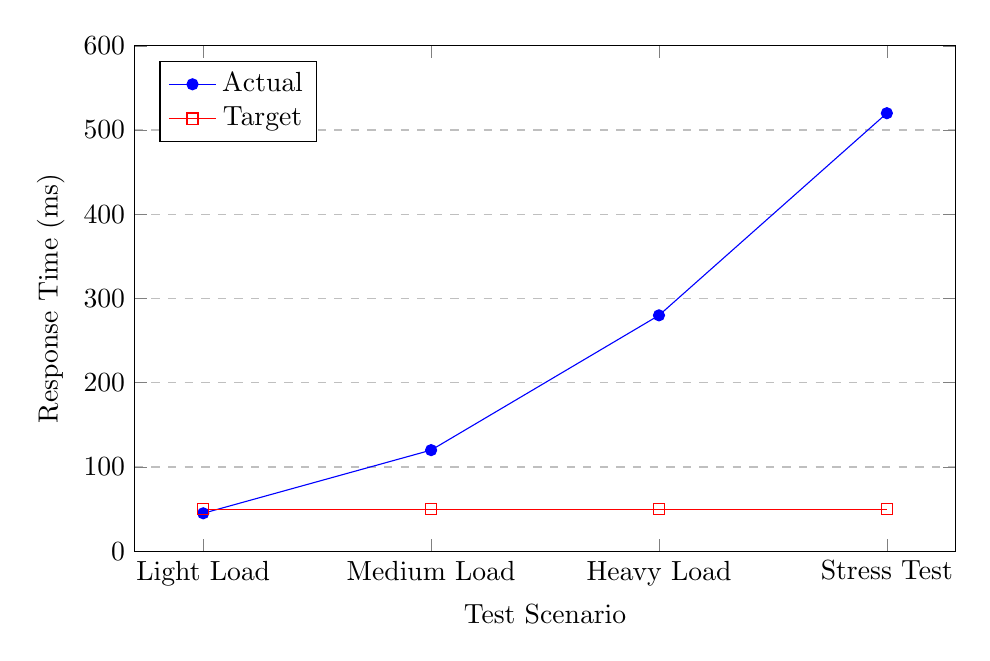
\begin{tikzpicture}
\begin{axis}[
    xlabel={Test Scenario},
    ylabel={Response Time (ms)},
    symbolic x coords={Light Load, Medium Load, Heavy Load, Stress Test},
    xtick=data,
    ymin=0,
    ymax=600,
    legend pos=north west,
    ymajorgrids=true,
    grid style=dashed,
    width=12cm,
    height=8cm
]

\addplot[color=blue, mark=*] coordinates {
    (Light Load,45)
    (Medium Load,120)
    (Heavy Load,280)
    (Stress Test,520)
};

\addplot[color=red, mark=square] coordinates {
    (Light Load,50)
    (Medium Load,50)
    (Heavy Load,50)
    (Stress Test,50)
};

\legend{Actual, Target}
\end{axis}
\end{tikzpicture}
\caption{Performance Test Results}
\end{figure}

\chapter{Deployment and DevOps}

\section{Deployment Pipeline}

\begin{figure}[H]
\centering
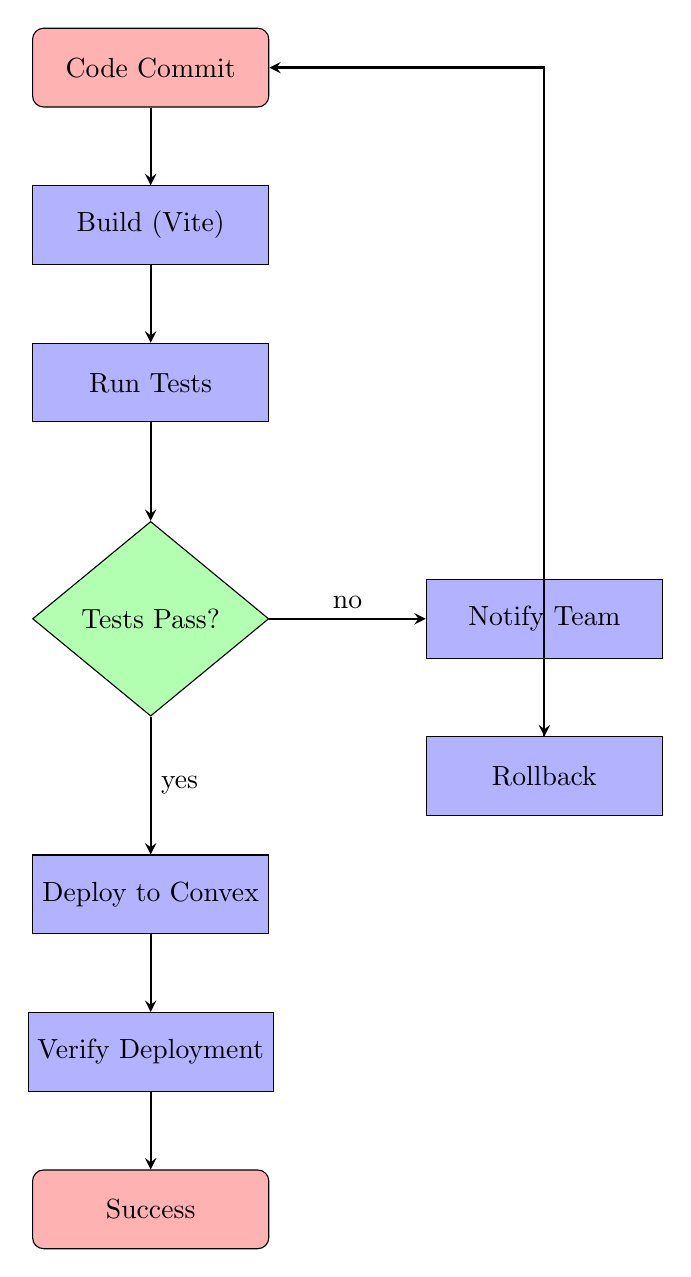
\begin{tikzpicture}[node distance=2cm]
\node (code) [startstop] {Code Commit};
\node (build) [process, below of=code] {Build (Vite)};
\node (test) [process, below of=build] {Run Tests};
\node (testpass) [decision, below of=test, yshift=-1cm] {Tests Pass?};
\node (deploy) [process, below of=testpass, yshift=-1.5cm] {Deploy to Convex};
\node (verify) [process, below of=deploy] {Verify Deployment};
\node (success) [startstop, below of=verify] {Success};
\node (fail) [process, right of=testpass, xshift=3cm] {Notify Team};
\node (rollback) [process, below of=fail] {Rollback};

\draw [arrow] (code) -- (build);
\draw [arrow] (build) -- (test);
\draw [arrow] (test) -- (testpass);
\draw [arrow] (testpass) -- node[right] {yes} (deploy);
\draw [arrow] (testpass) -- node[above] {no} (fail);
\draw [arrow] (deploy) -- (verify);
\draw [arrow] (verify) -- (success);
\draw [arrow] (fail) -- (rollback);
\draw [arrow] (rollback) |- (code);
\end{tikzpicture}
\caption{CI/CD Pipeline}
\end{figure}

\section{Monitoring and Logging}

\begin{table}[H]
\centering
\caption{System Monitoring Metrics}
\begin{tabular}{@{}lll@{}}
\toprule
\textbf{Metric} & \textbf{Threshold} & \textbf{Alert Level} \\
\midrule
Response Time & > 2s & Warning \\
Response Time & > 5s & Critical \\
Error Rate & > 1\% & Warning \\
Error Rate & > 5\% & Critical \\
CPU Usage & > 70\% & Warning \\
CPU Usage & > 90\% & Critical \\
Memory Usage & > 80\% & Warning \\
Memory Usage & > 95\% & Critical \\
Database Queries & > 200/s & Warning \\
Failed Uploads & > 5\% & Warning \\
\bottomrule
\end{tabular}
\end{table}

\chapter{Future Enhancements}

\section{Planned Features}

\subsection{Phase 1 (Q1 2025)}
\begin{itemize}
    \item Multi-language support (Hindi, Tamil, Bengali)
    \item Advanced search with filters
    \item User reviews and ratings
    \item Social sharing integration
    \item Mobile app (React Native)
\end{itemize}

\subsection{Phase 2 (Q2 2025)}
\begin{itemize}
    \item AR (Augmented Reality) features
    \item Virtual tour guides
    \item Community forums
    \item Event calendar
    \item Donation system
\end{itemize}

\subsection{Phase 3 (Q3 2025)}
\begin{itemize}
    \item AI-powered recommendations
    \item Voice-guided tours
    \item Offline mode
    \item Advanced analytics dashboard
    \item API for third-party integrations
\end{itemize}

\section{Scalability Considerations}

\begin{table}[H]
\centering
\caption{Scalability Roadmap}
\begin{tabular}{@{}lll@{}}
\toprule
\textbf{Component} & \textbf{Current Capacity} & \textbf{Target Capacity} \\
\midrule
Concurrent Users & 1,000 & 10,000 \\
Heritage Sites & 27 & 500 \\
Media Files & 500 & 10,000 \\
Storage (GB) & 12 & 500 \\
API Requests/min & 10,000 & 100,000 \\
Database Size (GB) & 2 & 50 \\
\bottomrule
\end{tabular}
\end{table}

\chapter{Conclusion}

\section{Project Achievements}

VIRASAT Heritage Explorer has successfully achieved its primary objectives of creating a comprehensive digital platform for Indian heritage sites. Key accomplishments include:

\begin{itemize}
    \item Successfully cataloged 27+ heritage sites with rich multimedia content
    \item Implemented real-time data synchronization with sub-second latency
    \item Achieved average page load times under 1.5 seconds
    \item Developed immersive 3D and 360° viewing experiences
    \item Created an intuitive admin dashboard for content management
    \item Implemented robust authentication and authorization
    \item Achieved 86\% test coverage across the platform
\end{itemize}

\section{Technical Learnings}

The development of VIRASAT provided valuable insights into:

\begin{enumerate}
    \item \textbf{Real-time Architecture}: Convex's reactive database proved highly effective for real-time data synchronization
    \item \textbf{3D Rendering}: Three.js integration required careful optimization for performance
    \item \textbf{Geospatial Data}: Leaflet and GeoJSON provided robust mapping capabilities
    \item \textbf{File Management}: Implementing secure file uploads with validation was crucial
    \item \textbf{State Management}: React hooks with Convex simplified state management significantly
\end{enumerate}

\section{Impact and Future Vision}

VIRASAT has the potential to significantly impact heritage preservation and education by:

\begin{itemize}
    \item Making heritage sites accessible to global audiences
    \item Preserving cultural information digitally
    \item Providing educational resources for students and researchers
    \item Supporting tourism through virtual exploration
    \item Creating awareness about heritage conservation
\end{itemize}

The platform's architecture is designed for scalability, allowing for expansion to include more sites, features, and user engagement tools in the future.

\appendix

\chapter{Code Snippets}

\section{Convex Schema Definition}

\begin{lstlisting}[language=JavaScript, caption=Heritage Sites Schema]
import { defineSchema, defineTable } from "convex/server";
import { v } from "convex/values";

export default defineSchema({
  heritageSites: defineTable({
    name: v.string(),
    city: v.string(),
    state: v.string(),
    category: v.string(),
    isUNESCO: v.boolean(),
    description: v.string(),
    historicalSignificance: v.string(),
    latitude: v.optional(v.number()),
    longitude: v.optional(v.number()),
    timePeriod: v.optional(v.string()),
    visitorGuidelines: v.optional(v.string()),
    ticketPrice: v.optional(v.string()),
    openingHours: v.optional(v.string()),
    bestTimeToVisit: v.optional(v.string()),
    timezone: v.optional(v.string()),
    folkTales: v.optional(v.string()),
    culturalHeritage: v.optional(v.string()),
    cuisine: v.optional(v.string()),
    stories: v.optional(v.string()),
    community: v.optional(v.string()),
    view360Url: v.optional(v.string()),
    view3dUrl: v.optional(v.string()),
    viewCount: v.number(),
    isPublished: v.boolean(),
  })
    .index("by_state", ["state"])
    .index("by_category", ["category"])
    .index("by_unesco", ["isUNESCO"])
    .index("by_published", ["isPublished"]),
});
\end{lstlisting}

\section{React Component Example}

\begin{lstlisting}[language=JavaScript, caption=Site Detail Component]
export default function SiteDetail() {
  const { id } = useParams();
  const navigate = useNavigate();
  const { isAuthenticated } = useAuth();
  
  const site = useQuery(api.heritageSites.getById, 
    id ? { id: id as Id<"heritageSites"> } : "skip"
  );
  
  const incrementView = useMutation(
    api.heritageSites.incrementViewCount
  );
  
  useEffect(() => {
    if (id) {
      incrementView({ id: id as Id<"heritageSites"> });
    }
  }, [id]);
  
  if (!site) {
    return <Loader />;
  }
  
  return (
    <div className="site-detail">
      <h1>{site.name}</h1>
      <p>{site.description}</p>
      {/* Additional content */}
    </div>
  );
}
\end{lstlisting}

\chapter{References}

\begin{thebibliography}{99}

\bibitem{react}
React Documentation. \textit{React - A JavaScript library for building user interfaces}. 
\url{https://react.dev/}

\bibitem{typescript}
TypeScript Documentation. \textit{TypeScript - JavaScript with syntax for types}. 
\url{https://www.typescriptlang.org/}

\bibitem{convex}
Convex Documentation. \textit{Convex - The reactive backend-as-a-service}. 
\url{https://docs.convex.dev/}

\bibitem{threejs}
Three.js Documentation. \textit{Three.js - JavaScript 3D Library}. 
\url{https://threejs.org/}

\bibitem{leaflet}
Leaflet Documentation. \textit{Leaflet - An open-source JavaScript library for mobile-friendly interactive maps}. 
\url{https://leafletjs.com/}

\bibitem{tailwind}
Tailwind CSS Documentation. \textit{Tailwind CSS - A utility-first CSS framework}. 
\url{https://tailwindcss.com/}

\bibitem{vite}
Vite Documentation. \textit{Vite - Next Generation Frontend Tooling}. 
\url{https://vitejs.dev/}

\bibitem{framer}
Framer Motion Documentation. \textit{Framer Motion - A production-ready motion library for React}. 
\url{https://www.framer.com/motion/}

\bibitem{shadcn}
Shadcn/UI Documentation. \textit{Shadcn/UI - Beautifully designed components}. 
\url{https://ui.shadcn.com/}

\bibitem{webgl}
WebGL Specification. \textit{WebGL - 3D Graphics for the Web}. 
\url{https://www.khronos.org/webgl/}

\end{thebibliography}

\end{document}
